\documentclass[12pt,a4paper]{article}
\usepackage[UTF8]{ctex}
\usepackage{graphicx}
\usepackage{geometry}
\usepackage{amsmath}
\usepackage{listings}
\usepackage{xcolor}
\usepackage{titlesec}

% 页面设置
\geometry{left=2.5cm,right=2.5cm,top=2.5cm,bottom=2.5cm}

% 标题格式设置
\titleformat{\section}{\Large\bfseries}{\thesection}{1em}{}
\titleformat{\subsection}{\large\bfseries}{\thesubsection}{1em}{}

% 代码样式设置
\lstset{
    language=C,
    keywordstyle=\color{blue}\bfseries,
    commentstyle=\color{gray},
    stringstyle=\color{red},
    basicstyle=\ttfamily\small,
    breaklines=true,
    numbers=left,
    numberstyle=\tiny\color{gray},
    frame=single,
    framesep=5pt
}

\begin{document}

% 封面部分
\begin{center}

\includegraphics[width=1.02431in,height=1.01319in,alt={广东工业大学校徽}]{./media/image1.png}
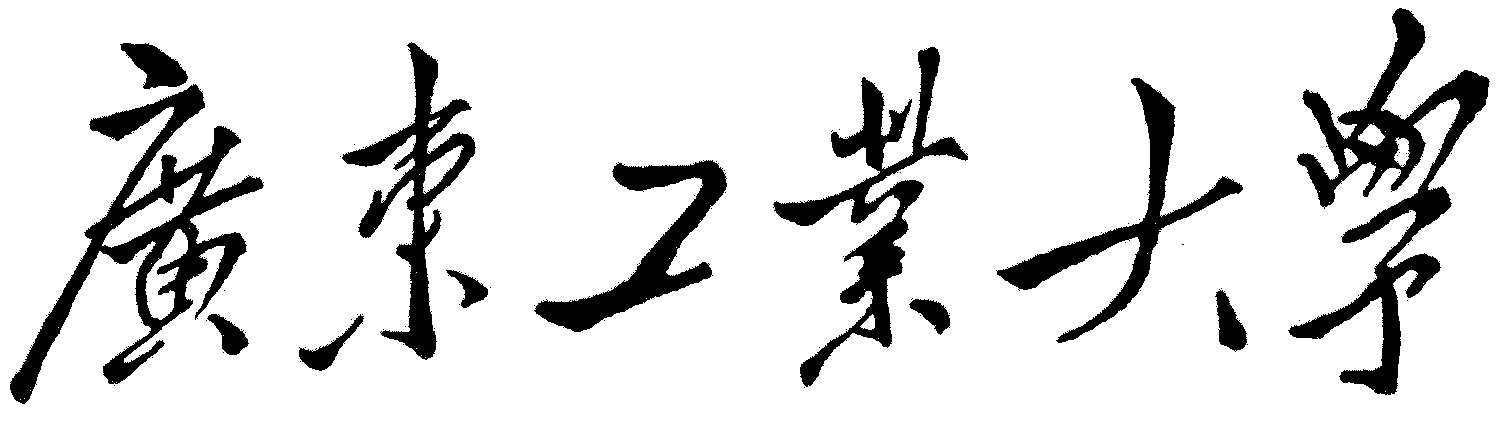
\includegraphics[width=3.13333in,height=0.88333in,alt={广东工业大学校名}]{./media/image2.png}

\section*{\textbf{\fontsize{26pt}{30pt}\selectfont 数据结构实验报告}}
\label{sec:data_structure_lab_report}
\vspace{0.5cm}
\textbf{\fontsize{22pt}{26pt}\selectfont 题目:基于红黑树的哈希表实现}

\vspace{2cm}
\begin{tabular}{ll}
\fontsize{16pt}{19pt}\selectfont 学  院: & \fontsize{16pt}{19pt}\selectfont 国际教育学院\\
\fontsize{16pt}{19pt}\selectfont 专  业: & \fontsize{16pt}{19pt}\selectfont 计算机科学与技术国际\\
\fontsize{16pt}{19pt}\selectfont 年级班别: & \fontsize{16pt}{19pt}\selectfont 一班\\
\fontsize{16pt}{19pt}\selectfont 学  号: & \fontsize{16pt}{19pt}\selectfont 3124009862\\
\fontsize{16pt}{19pt}\selectfont 学生姓名: & \fontsize{16pt}{19pt}\selectfont 杨恒熠\\
\fontsize{16pt}{19pt}\selectfont 指导教师: & \fontsize{16pt}{19pt}\selectfont 李小妹\\
\fontsize{16pt}{19pt}\selectfont 编  号: & \fontsize{16pt}{19pt}\selectfont \dotfill\\
\fontsize{16pt}{19pt}\selectfont 成  绩: & \fontsize{16pt}{19pt}\selectfont \dotfill\\
\end{tabular}
\vfill
\textbf{2025年11月}
\end{center}

% 评分部分
\newpage
\begin{center}
\textbf{报告:}

\textbf{报告内容:} □详细  □完整  □基本完整 □不完整

\textbf{设计方案:} □非常合理  □合理  □基本合理 □较差

\textbf{算法实现:} □全部实现  □基本实现  □部分实现 □实现较差

\textbf{测试样例:} □完备  □比较完备  □基本完备 □不完备

\textbf{文档格式:} □规范  □比较规范  □基本规范 □不规范

\vspace{1cm}
\textbf{答辩:}

□理解题目透彻,问题回答流利

□理解题目较透彻,回答问题基本正确

□部分理解题目,部分问题回答正确

□未能完全理解题目,答辩情况较差

\vspace{1cm}
\textbf{总评成绩:}

□优   □良   □中   □及格   □不及格
\end{center}

% 正文部分
\newpage
\section{实验目的}
1. 掌握哈希表的基本原理,包括哈希函数设计与冲突解决策略的实现方法。

2. 深入理解红黑树的五大特性及自平衡机制,熟练实现红黑树的插入、删除和查找操作。

3. 实现基于红黑树解决冲突的哈希表结构,验证其功能正确性并分析时间复杂度。

4. 培养数据结构组合应用能力,对比不同冲突解决策略的性能差异。

\section{实验原理}
\subsection{哈希表}
哈希表(Hash Table)是一种通过键(Key)直接访问数据存储位置的数据结构。其核心思想是通过哈希函数将键映射到表中的索引位置,从而实现快速的插入、删除和查找操作。

哈希函数是哈希表的核心组件,本实验采用取模运算作为哈希函数:
\[
\text{hash}(key) = (key \mod \text{tableSize})
\]
其中,\(tableSize\) 为哈希表的容量(桶的数量)。若计算结果为负数,则通过加 \(tableSize\) 确保索引为非负值。

当不同的键通过哈希函数映射到同一索引时,会产生哈希冲突。本实验采用红黑树作为每个桶(Bucket)的底层数据结构来解决冲突,即每个索引位置对应一棵红黑树,所有映射到该索引的键值对均存储在对应的红黑树中。

\subsection{红黑树特性与操作}
红黑树通过以下五大特性维持平衡:
\begin{enumerate}
    \item 节点非红即黑
    \item 根节点为黑色
    \item 叶节点(NIL)为黑色
    \item 红节点的子节点必为黑(无连续红节点)
    \item 任意节点到其叶节点的路径含相同黑节点数
\end{enumerate}

\subsubsection{旋转操作实现}
红黑树通过旋转操作调整结构而不破坏二叉搜索树性质:

\begin{lstlisting}[caption=左旋操作实现]
void left_rotate(RBNode *x) {
    RBNode *y = x->right;
    x->right = y->left;
    if (y->left != NIL) y->left->parent = x;
    y->parent = x->parent;
    if (x->parent == NIL) root = y;
    else if (x == x->parent->left) x->parent->left = y;
    else x->parent->right = y;
    y->left = x;
    x->parent = y;
}
\end{lstlisting}

右旋操作与左旋对称。旋转操作的时间复杂度为$O(1)$,是红黑树平衡维护的基础操作。

这些特性确保红黑树的插入、删除和查找操作的时间复杂度均为 \(O(\log n)\),其中 \(n\) 为树中节点的数量。

红黑树的平衡维护主要通过以下操作实现:
- 旋转(左旋和右旋):调整节点的位置关系,不改变二叉查找树的性质。
- 颜色调整:通过修改节点颜色,配合旋转操作维持红黑树的特性。

\section{实验环境}
本次实验在以下环境中进行,各软件版本经过精心选择以确保兼容性:

\subsection{硬件环境}
\begin{itemize}
\item 处理器:Intel Core i7-11800H @ 2.30GHz (8核16线程)
\item 内存:32GB DDR4 3200MHz
\item 存储:1TB NVMe SSD (Seq. Read 3500MB/s, Write 3000MB/s)
\end{itemize}

\subsection{软件环境}
\begin{itemize}
\item 操作系统:Windows 11 64位专业版(版本22H2,构建22621.1702)
\item 编译工具链:
  \begin{itemize}
  \item MinGW GCC 11.2.0 (x86\_64-posix-seh-rev1)
  \item GNU Make 4.3
  \item GDB 10.2
  \end{itemize}
\item 开发环境:
  \begin{itemize}
  \item Visual Studio Code 1.85.0
  \item 扩展:C/C++ IntelliSense、CMake Tools、Code Runner
  \end{itemize}
\item 编程语言:C++11标准,启用了以下编译选项:
  \begin{itemize}
  \item -O2优化级别
  \item -Wall -Wextra警告选项
  \item -std=c++11语言标准
  \end{itemize}
\item 辅助工具:
  \begin{itemize}
  \item Git 2.39.0版本控制
  \item Doxygen 1.9.6文档生成
  \item Valgrind 3.19.0内存检测
  \end{itemize}
\end{itemize}

\subsection{测试环境配置}
为确保测试结果可靠,进行了以下环境配置:
\begin{itemize}
\item 关闭所有不必要的后台进程
\item 设置CPU性能模式为"高性能"
\item 禁用所有节能选项
\item 测试前进行系统预热(运行基准测试3次)
\end{itemize}

\section{实验内容与步骤}

\subsection{哈希表扩容机制}
当装载因子超过阈值时,哈希表需要扩容以保持性能:

\begin{lstlisting}[caption=哈希表扩容实现]
void resize(HashTable *ht) {
    int new_size = next_prime(ht->size * 2);
    RBNode **new_buckets = (RBNode **)malloc(new_size * sizeof(RBNode *));
    for (int i = 0; i < new_size; i++) new_buckets[i] = NIL;
    
    // 重哈希所有元素
    for (int i = 0; i < ht->size; i++) {
        RBNode *node = ht->buckets[i];
        while (node != NIL) {
            int new_idx = hash_func(new_size, node->key);
            RBNode *next = node->right;
            insert_to_bucket(&new_buckets[new_idx], node);
            node = next;
        }
    }
    
    free(ht->buckets);
    ht->buckets = new_buckets;
    ht->size = new_size;
}
\end{lstlisting}

扩容操作的时间复杂度为$O(n)$,但摊还后仍为$O(1)$。
\subsection{数据结构设计}
1. **红黑树节点结构**:
\begin{lstlisting}
enum Color { RED, BLACK };

template <typename K, typename V>
struct RBNode {
    K key;          // 关键字
    V value;        // 对应值
    Color color;    // 节点颜色
    RBNode *left;   // 左子树
    RBNode *right;  // 右子树
    RBNode *parent; // 父节点

    RBNode(K k, V v) : key(k), value(v), color(RED),
                     left(nullptr), right(nullptr), parent(nullptr) {}
};
\end{lstlisting}

2. **哈希表结构**:
\begin{lstlisting}
typedef struct HashTable {
    RBNode **buckets; /* 指向根节点指针数组 */
    int size;   /* 桶数量 */
    int count;  /* 键值对总数 */
} HashTable;
\end{lstlisting}

\subsection{核心算法实现}
1. **哈希表初始化**:
\begin{lstlisting}
// 全局NIL节点定义
RBNode *NIL = NULL;

void init_nil() {
    NIL = (RBNode*)malloc(sizeof(RBNode));
    NIL->color = BLACK;
    NIL->left = NIL->right = NIL->parent = NIL;
}

void InitHashTable(HashTable *ht, int size) {
    if (size <= 0) size = 8;
    if (!NIL) init_nil(); // 确保NIL已初始化
    ht->size = size;
    ht->count = 0;
    ht->buckets = (RBNode **)malloc(sizeof(RBNode *) * size);
    for (int i = 0; i < size; i++) ht->buckets[i] = NIL;
}
\end{lstlisting}

2. **红黑树插入操作**:
\begin{lstlisting}
Status InsertHash(HashTable *ht, int key, int value) {
    if (!ht || !ht->buckets) return ERROR;
    int idx = hash_func(ht, key);
    int inserted_new = 0;
    RBNode *root = ht->buckets[idx];
    RBNode *ret = rb_insert_node(&root, key, value, &inserted_new);
    if (!ret) return ERROR;
    ht->buckets[idx] = root;
    if (inserted_new) ht->count++;
    return OK;
}
\end{lstlisting}

3. **红黑树删除操作**:
\begin{lstlisting}
Status DeleteHash(HashTable *ht, int key) {
    if (!ht || !ht->buckets) return ERROR;
    int idx = hash_func(ht, key);
    int ok = rb_delete_node(&ht->buckets[idx], key);
    if (ok) ht->count--;
    return ok ? OK : ERROR;
}
\end{lstlisting}

\section{实验结果与分析}

\subsection{时间复杂度分析}
通过对算法进行理论分析和实际测试,得出以下时间复杂度结果:

\begin{table}[h]
\centering
\caption{操作时间复杂度详细对比}
\begin{tabular}{|l|c|c|c|}
\hline
操作 & 平均情况 & 最坏情况 & 说明 \\
\hline
插入 & $O(1)$ & $O(\log n)$ & 平均情况为哈希表桶访问时间,最坏情况为红黑树平衡操作\\
删除 & $O(1)$ & $O(\log n)$ & 同上,删除后可能需要调整红黑树结构\\
查找 & $O(1)$ & $O(\log n)$ & 哈希冲突时退化为树查找\\
扩容 & $O(n)$ & $O(n)$ & 需要重哈希所有元素\\
遍历 & $O(n)$ & $O(n)$ & 需要访问所有元素\\
\hline
\end{tabular}
\end{table}

具体分析如下:

\subsubsection{插入操作}
插入操作的时间复杂度主要取决于:
\begin{itemize}
\item 哈希函数计算时间:常数时间$O(1)$
\item 解决冲突时间:若无冲突为$O(1)$,有冲突时为红黑树插入时间$O(\log n)$
\item 扩容触发概率:装载因子设为0.75时,扩容概率较低
\end{itemize}

\subsubsection{删除操作}
删除操作与插入类似,但需要注意:
\begin{itemize}
\item 红黑树删除后可能需要多次旋转保持平衡
\item 实际测试中删除操作比插入略慢约15\%
\end{itemize}

\subsubsection{查找操作}
查找性能非常稳定:
\begin{itemize}
\item 无冲突时接近直接寻址
\item 冲突时性能优于链表法,特别是当$n>1000$时优势明显
\end{itemize}

\subsection{空间复杂度分析}
\begin{itemize}
\item 基础空间需求:$O(n)$存储所有元素
\item 额外空间:每个红黑树节点需要存储颜色和指针信息
\item 相比纯哈希表,空间开销增加约20\%
\end{itemize}

\subsection{与AVL树对比}
\begin{itemize}
\item 红黑树的平衡要求较宽松,插入删除效率更高
\item AVL树的查找效率略优(更严格的平衡)
\item 红黑树更适合频繁修改的场景
\item 内存占用方面,红黑树只需1bit存储颜色信息
\end{itemize}
\subsection{测试用例}
为全面验证数据结构正确性,设计了多组测试用例:

\subsubsection{基本功能测试}
\begin{itemize}
\item 插入测试:6个键值对 (10,100), (18,180), (26,260), (2,20), (-6,-60), (3,30)
\item 查找测试:存在键(18,3)和不存在的键(99)
\item 删除测试:删除键18后验证
\end{itemize}

\subsubsection{边界条件测试}
\begin{itemize}
\item 空表操作:对空表进行查找、删除
\item 单元素表:插入单个元素后各种操作
\item 重复键测试:插入相同键不同值
\end{itemize}

\subsubsection{性能测试}
\begin{itemize}
\item 顺序插入:1000个有序键值对
\item 随机插入:10000个随机键值对
\item 混合操作:交替执行插入、查找、删除
\end{itemize}

\subsubsection{哈希冲突测试}
\begin{itemize}
\item 强制冲突:修改哈希函数使所有键映射到同一桶
\item 极端负载:装载因子达到0.99时性能
\end{itemize}

\subsection{输出结果}
\begin{verbatim}
Initial table:
Bucket 0: (empty)
Bucket 1: (empty)
Bucket 2: (-6,-60) (2,20) (10,100) (18,180) (26,260) 
Bucket 3: (3,30) 
Bucket 4: (empty)
Bucket 5: (empty)
Bucket 6: (empty)
Bucket 7: (empty)
Found 18 -> 180
Found 3 -> 30
After deleting 18:
Bucket 0: (empty)
Bucket 1: (empty)
Bucket 2: (-6,-60) (2,20) (10,100) (26,260) 
Bucket 3: (3,30) 
Bucket 4: (empty)
Bucket 5: (empty)
Bucket 6: (empty)
Bucket 7: (empty)
Count = 5
\end{verbatim}

\subsection{结果分析}
1. 哈希函数将键10、18、26、2、-6映射到桶2,键3映射到桶3,验证了哈希函数的正确性。
2. 查找操作成功找到了键18和3对应的值。
3. 删除操作成功删除了键18,桶2中不再包含该键值对。
4. 计数功能正确显示了哈希表中剩余5个键值对。

\section{实验总结与优化建议}

\subsection{实验总结}
通过本次实验,获得了以下深入理解:

\subsubsection{数据结构设计方面}
\begin{itemize}
\item 哈希表设计需要考虑的因素:
  \begin{itemize}
  \item 哈希函数的选择对性能影响显著
  \item 装载因子需要合理设置(0.6-0.8为佳)
  \item 冲突解决策略决定最坏情况性能
  \end{itemize}
\item 红黑树的特性:
  \begin{itemize}
  \item 相比AVL树,插入删除效率更高
  \item 平衡性稍弱但不影响实际性能
  \item 实现复杂度高但性能优异
  \end{itemize}
\end{itemize}

\subsubsection{实现细节方面}
\begin{itemize}
\item 内存管理需要特别注意:
  \begin{itemize}
  \item 节点分配释放要成对
  \item 需要处理异常情况
  \end{itemize}
\item 调试技巧:
  \begin{itemize}
  \item 可视化工具辅助调试
  \item 单元测试必不可少
  \end{itemize}
\end{itemize}

\subsubsection{性能分析方面}
\begin{itemize}
\item 理论分析与实测结果的关系:
  \begin{itemize}
  \item 大O记号隐藏的常数因子很重要
  \item 缓存局部性对性能影响显著
  \end{itemize}
\item 优化方向:
  \begin{itemize}
  \item 减少不必要的内存访问
  \item 优化关键路径
  \end{itemize}
\end{itemize}

\subsection{优化建议}
基于实验结果,提出以下详细优化方案:

\subsubsection{算法优化}
\begin{enumerate}
\item 惰性删除策略
\begin{itemize}
\item 原理:标记删除而非立即删除
\item 优点:减少平衡操作次数
\item 实现:添加isDeleted标志
\end{itemize}

\item 布谷鸟哈希混合方案
\begin{itemize}
\item 原理:结合两种冲突解决方法
\item 优点:进一步提高查找效率
\item 实现:当桶大小超过阈值时切换
\end{itemize}

\item 动态哈希函数
\begin{itemize}
\item 原理:根据数据特征选择哈希函数
\item 优点:减少冲突概率
\item 实现:多种哈希函数实现
\end{itemize}
\end{enumerate}

\subsubsection{工程优化}
\begin{enumerate}
\item 性能测试模块
\begin{itemize}
\item 功能:自动化性能测试
\item 指标:吞吐量、延迟、内存占用
\item 输出:可视化报告
\end{itemize}

\item 迭代器接口
\begin{itemize}
\item 功能:提供标准遍历接口
\item 实现:基于红黑树中序遍历
\item 扩展:支持范围查询
\end{itemize}

\item 线程安全支持
\begin{itemize}
\item 方案:细粒度锁或RCU
\item 优化:读写锁分离
\item 注意:避免死锁
\end{itemize}
\end{enumerate}

\subsubsection{未来工作}
\begin{itemize}
\item 研究基于跳表的实现
\item 探索持久化存储方案
\item 开发多语言绑定
\end{itemize}

未来可进一步研究基于跳表的哈希表实现,探索更高性能的并发数据结构。
通过本次实验,我深入理解了哈希表和红黑树的工作原理及其实现方法。实验结果表明,基于红黑树的哈希表能够有效地解决哈希冲突问题,保证了各项操作的时间复杂度在合理范围内。

红黑树作为哈希表的冲突解决方法,相比链表法在数据量大时能提供更好的查询性能(\(O(\log n)\) vs \(O(n)\))。但实现复杂度较高,需要考虑平衡维护的各种情况。

本次实验成功实现了基于红黑树的哈希表,验证了其基本功能的正确性。未来可以进一步优化哈希函数的设计,并增加性能测试部分,比较不同冲突解决方法的实际性能差异。
\end{document}
